\documentclass[10pt, aspectratio=169]{beamer}

\usepackage{appendixnumberbeamer}

\usepackage[utf8]{inputenc}
\usepackage{lmodern,mathtools,amsmath,amssymb}

\usepackage{tikz}
\usepackage{xcolor}
\definecolor{title}{rgb}{.2, .2, .7}

\usetikzlibrary{arrows, arrows.meta, decorations.pathreplacing, bending}

\AtBeginSection[]{
    \begin{frame}
        \huge \centering \color{title}\insertsectionhead\par
    \end{frame}
}

\usepackage{amsmath}
\usepackage{amsfonts}
\usepackage{amssymb}
\usepackage{physics}
\usepackage{hyperref}

\usefonttheme[onlymath]{serif}
\setbeamercovered{invisible}

\title{\Huge Komplexe Wechselstromkreise}
\date{\Large \today}
\author{\Large Philip Geißler, Kamal Abdellatif}

\setbeamertemplate{navigation symbols}{}


\begin{document}

\begin{frame}
	\titlepage
\end{frame}

\section{Wechselstromkreise}
\Large 
\begin{frame}
    \centering
    \visible<2->{
    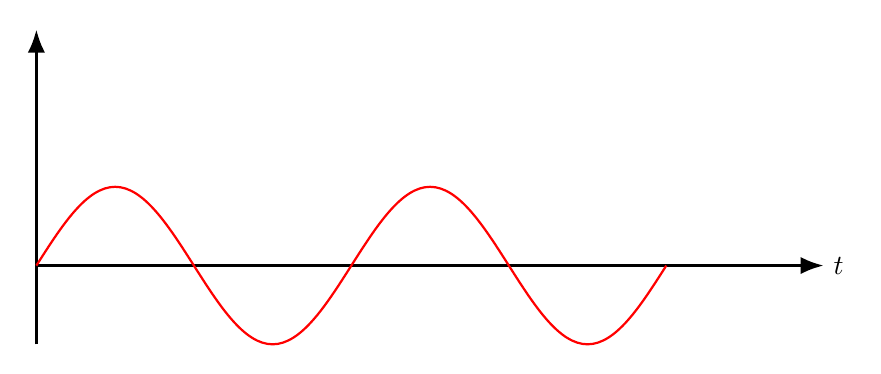
\begin{tikzpicture}
        \path[very thick, -{Latex}] (0, 0) edge (10, 0) (0, -1) edge (0, 3);
        \node[right] at (10, 0) {$t$};
        \draw[thick, red] (0, 0) sin (1, 1) cos (2, 0)
            sin (3, -1) cos (4, 0)
            sin (5, +1) cos (6, 0)
            sin (7, -1) cos (8, 0);
    \end{tikzpicture}
    }
    \\
    \visible<3>{
        \[ A(t) = \hat A\sin(\omega t + \phi) \]
    }
\end{frame}

\section{Die Bauteile}
\begin{frame}{Widerstand}
    \centering\Huge
    \visible<1->{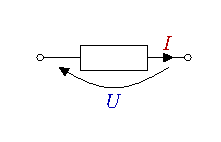
\includegraphics[width=.5\textwidth]{../script/kBR.pdf}}
    \visible<2->{
        $$U = R\cdot I$$
    }
\end{frame}
\begin{frame}{Widerstand}
    \centering\Huge
    \begin{align*}
        U(t) &= R \cdot I(t) \\
        \visible<2->{U(t) &= R \cdot \hat I\sin(\omega t)}
    \end{align*}
    \visible<3>{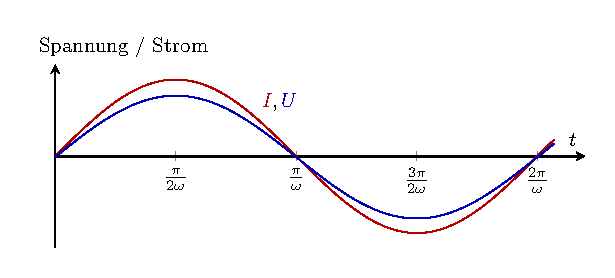
\includegraphics[width=.7\textwidth]{../script/kPR.pdf}}
\end{frame}
\begin{frame}{Kondensator}
    \centering\Huge
    \visible<1->{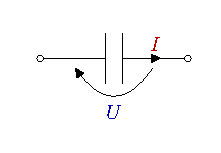
\includegraphics[width=.5\textwidth]{../script/kBC.pdf}}
    \visible<2->{
        \[ I = C\dot U \]
    }
\end{frame}
\begin{frame}{Kondensator}
    \begin{columns}
        \begin{column}{.25\textwidth}
           \begin{align*}
                \visible<1->{I(t) &= C \dv{t} U(t) \\}
                \visible<2->{I(t) &= C \dv{t} \hat U \sin(\omega t - \pi/2) \\}
                \only<-2>{\vphantom{\underbrace{}_{\hat I}}\\}
                \only<3>{I(t) &= \vphantom{\underbrace{}_{\hat I}}
                    \omega C \cdot \hat U \sin(\omega t)\\}
                \only<4->{I(t) &= \underbrace{\omega C \cdot \hat U}_{\hat I} \sin(\omega t)\\}
                \visible<5->{U(t) &= \frac1{\omega C}\cdot\hat I \sin(\omega t - \pi/2)}
            \end{align*}         
        \end{column}
        \begin{column}{.7\textwidth}
            \visible<6>{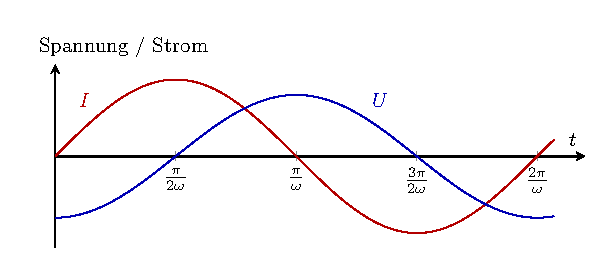
\includegraphics[width=\textwidth]{../script/kPC.pdf}}
        \end{column}
    \end{columns}
\end{frame}
\begin{frame}{Spule}
    \centering\Huge
    \visible<1->{\includegraphics[width=.5\textwidth]{../script/kBL.pdf}}
    \visible<2->{
        \[ U = L\dot I \]
    }
\end{frame}
\begin{frame}{Spule}
    \begin{columns}
        \begin{column}{.25\textwidth}
           \begin{align*}
                \visible<1->{U(t) &= L \dv{t} I(t) \\}
                \visible<2->{U(t) &= L \dv{t} \hat I \sin(\omega t) \\}
                \visible<3->{U(t) &= \omega L \cdot \hat I \sin(\omega t + \pi/2)}
            \end{align*}         
        \end{column}
        \begin{column}{.7\textwidth}
            \visible<3>{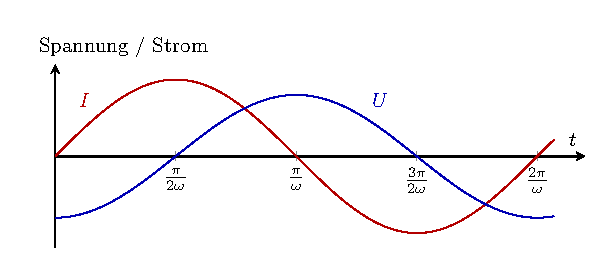
\includegraphics[width=\textwidth]{../script/kPC.pdf}}
        \end{column}
    \end{columns}
\end{frame}

\begin{frame}
    \centering\huge
    \begin{tabular}{r|cc}
        Bauteil & $\qquad\hat U / \hat I\qquad$ & $\phi$ \\\\
        \hline
        Widerstand & $R$ & $0$ \\\\
        Kondensator & ${1/\omega C}$ & $-\pi/2$ \\\\
        Spule & $\omega L$ & $+\pi/2$
    \end{tabular}
\end{frame}
\section{Zeigerdiagramme}
\begin{frame}
    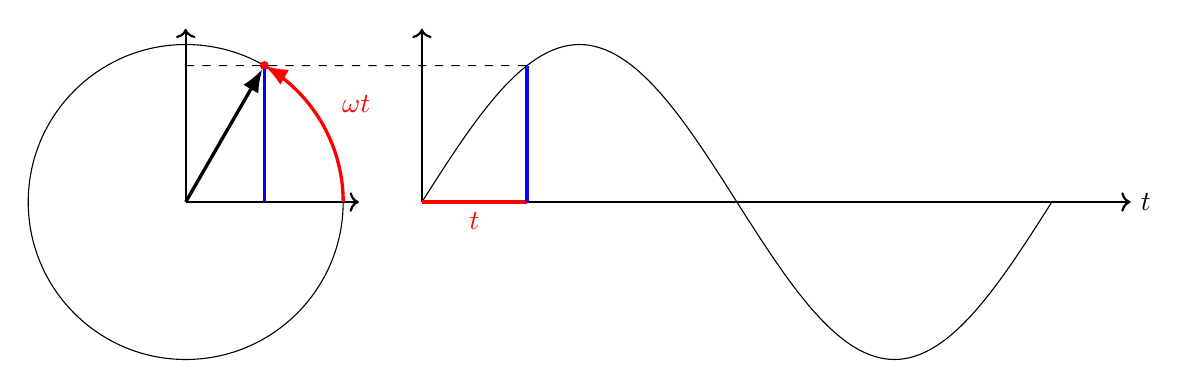
\begin{tikzpicture}
        \coordinate (M) at (-3, 0);
        \path (M) -- ++(60:2) node[inner sep=1pt] (P) {};

        \draw[thick, ->] (0, 0) -- +(0, 2.2);
        \draw[thick, ->] (0, 0) -- (9, 0) node[right] {$t$};

        \draw (0, 0) sin (2, 2) cos (4, 0)
            (8, 0) sin (6, -2) cos (4, 0);

        \visible<2->{
            \draw (M) circle (2);
            \draw[thick, ->] (M) -- +(2.2, 0);
            \draw[thick, ->] (M) -- +(0, 2.2);
        }

        \visible<3->{
            \draw[very thick, black, -{Latex}] (M) -- (P);
        }

        \visible<4->{
            \node[draw,red,shape=circle,fill=red,inner sep=1pt] at (P) {};
            \draw[very thick, red, -{Latex[flex=0]}] (-1, 0) arc (0:60:2);
            \path (M) -- ++(30:2.5) node[red] {$\omega t$};
            \draw[very thick, red] (0, 0) -- node[below,red] {$t$} (1.333, 0);
        }

        \visible<5>{
            \draw[very thick, blue] (-2, 0) -- (P)
                (1.333, 0) -- +(0, 1.732);
            \draw[dashed] (P)++(-1, 0) -- (1.333, 1.732);
        }
    \end{tikzpicture}
\end{frame}

\begin{frame}
    \centering
    \begin{tikzpicture}
        \definecolor{darkblue}{rgb}{0, 0, 0.7}
        \definecolor{darkgreen}{rgb}{0, 0.7, 0}
        \definecolor{darkred}{rgb}{0.7, 0, 0}
        \draw[thick, ->] (-4, 0) -- (4, 0);
        \draw[thick, ->] (0, -4) -- (0, 4);

        \visible<2->{
            \draw[ultra thick, -{Latex}, darkgreen] (0, 0) --
            node[above] {$R$} (0:3) node[above right] {$\mathbf{R}$};
        }
        \visible<3->{
            \draw[ultra thick, -{Latex}, darkred] (0, 0) --
            node[left] {$\omega L$} (90:3) node[above right] {$\mathbf{L}$};
        }
        \visible<4->{
            \draw[ultra thick, -{Latex}, darkblue] (0, 0) -- 
            node[left] {$1/\omega C$} (-90:3) node[below right] {$\mathbf{C}$};
        }
    \end{tikzpicture}
\end{frame}

\subsection{Komplexe Zahlen}
Normalerweise werden komplexe Zahlen via der imaginären Einheit $\imu^2 \coloneqq -1$ eingeführt.
Anschließend definiert man dann die komplexen Zahlen über $\mathbb{C} \ni c \coloneqq a + b\cdot \imu$ mit $a,b \in \mathbb{R}$.
Aus dieser Herangehensweise folgen dann recht schnell die Regeln zum Rechnen mit ebendiesen.
\begin{align*}
    c_1 +c_2 &= (a_1 + b_1\cdot \imu) + (a_2 + b_2\cdot \imu) &
    c_1 \cdot c_2 &= (a_1 + b_1\cdot \imu) \cdot (a_2 + b_2\cdot \imu) \\
        &= (a_1 + a_2) + (b_1 + b_2)\cdot \imu  &
        &= a_1a_2 + b_1b_2 \cdot \imu^2 + a_1b_2 \cdot \imu + a_2b_1 \cdot \imu\\
        &&&= (a_1a_2 - b_1b_2) + (a_1b_2 + a_1b_2) \cdot \imu
\end{align*}

\begin{wrapfigure}{r}{0.4\textwidth}
  \begin{centering}
    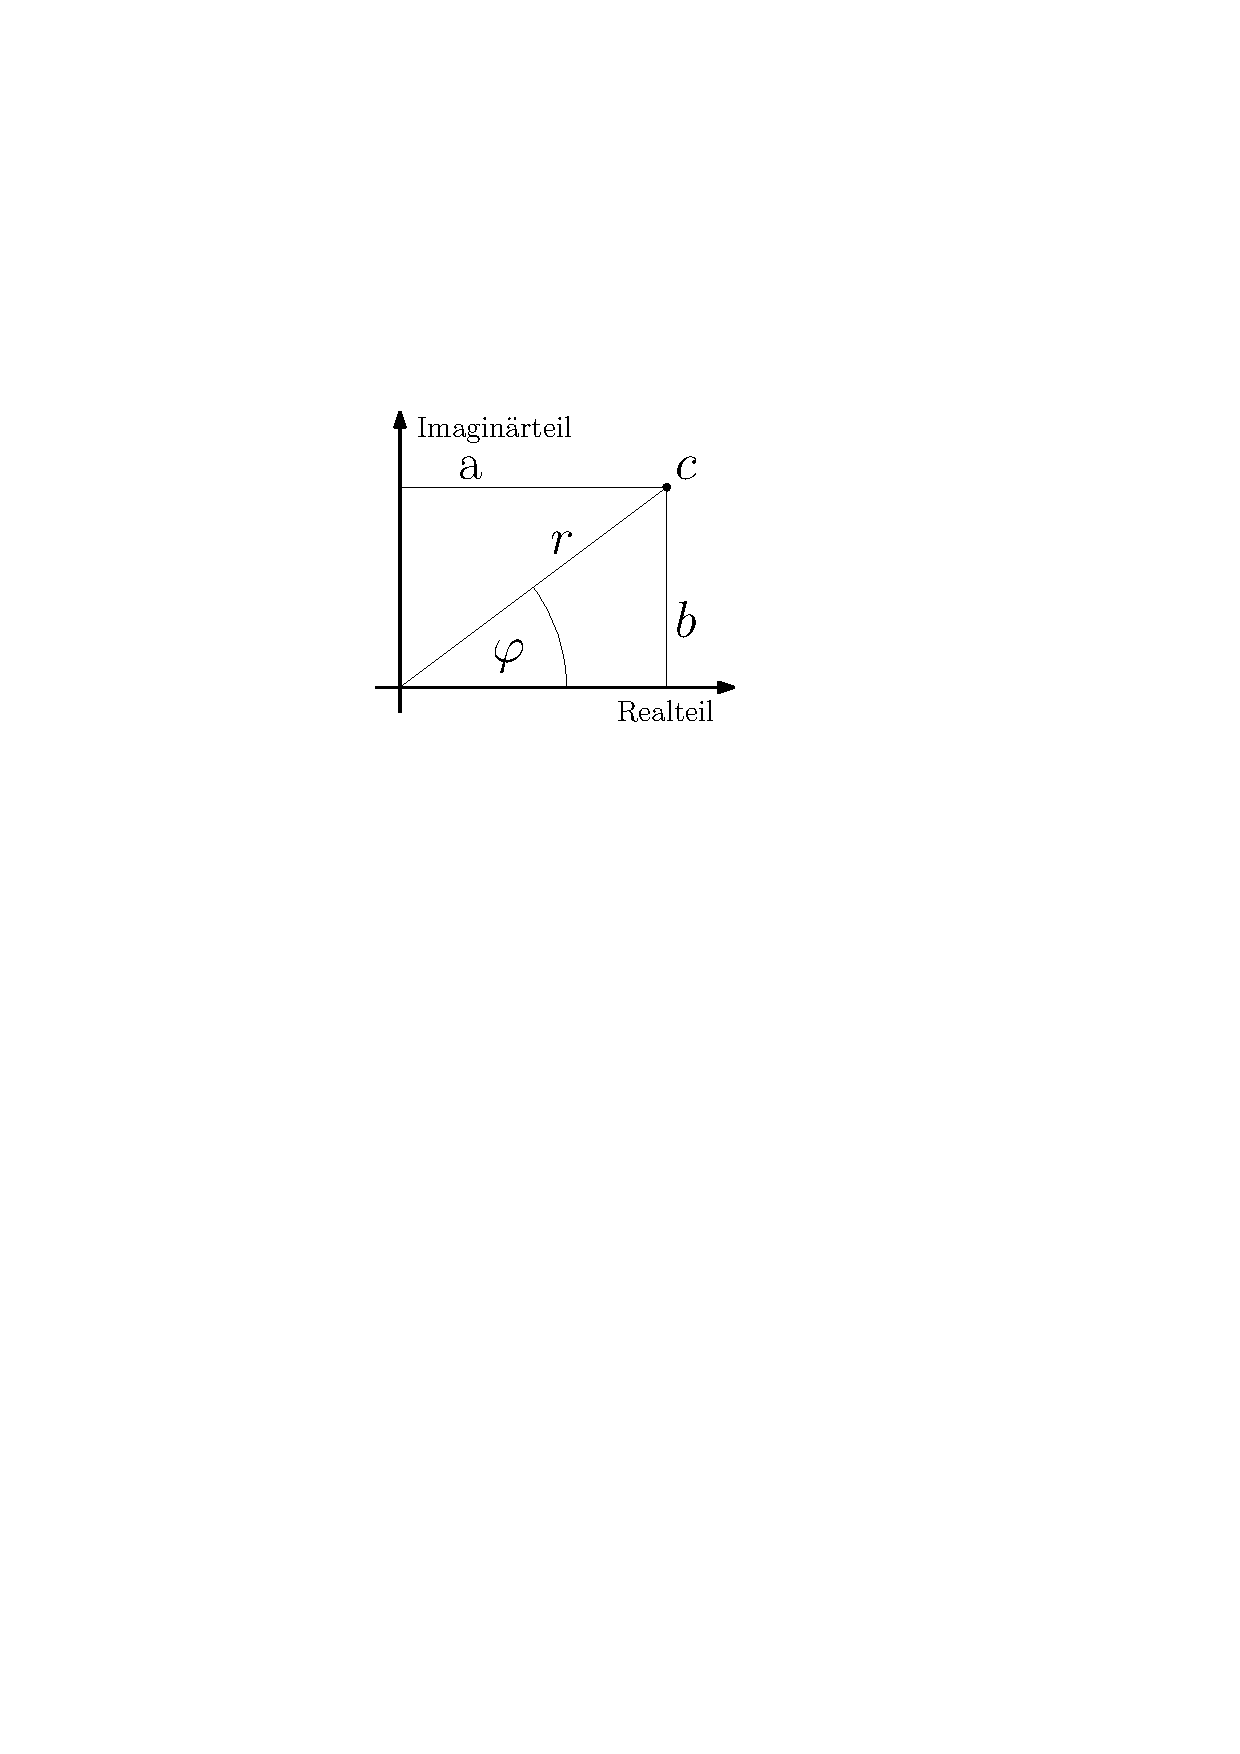
\includegraphics[width=0.4\textwidth]{philip1.pdf}
  \end{centering}
  \caption{Komplexe Zahl $c$ in kartesischen und polaren Koordinaten}
\end{wrapfigure}

Für den Anwendungsbereich der Wechselstromberechnungen ist es jedoch sinnvoller, komplexe Zahlen als
Repräsentanten von Punkten im zweidimensionalen Raum zu sehen, welche über die oben genannten Rechenvorschriften nützliche Eigenschaften besitzen, auf die im folgenden eingegangen werden soll.

Man denke sich eine komplexe Zahl $a +b\imu$ als einen Vektor $(a,\,b)_{x,y}$ im kartesischen Koordinatensystem mit X- und Y-Achse.
Dann sieht man, dass die Addition zweier komplexer Zahlen genau der Vektoraddition entspricht.
Weiterhin kann man den Vektor auch in einem polaren Koordinatensystem darstellen, in dem man aus $a$ und $b$ den 
Abstand zum Koordinatenursprung $r$ und den Winkel zur X-Achse $\varphi$ berechnet. Diese Form führt zu einer deutlich einprägsameren Multiplikationsformel.  
\begin{align*}
    a&=r \cdot \cos(\varphi) & c_1 &= a_1+b_1\imu = r_1\cos(\varphi_1) + r_1\sin(\varphi_1)\imu  \\
    b&=r \cdot \sin(\varphi) & c_2 &= a_2+b_2\imu = r_2\cos(\varphi_2) + r_2\sin(\varphi_2)\imu
\end{align*} \vspace*{-5mm}
\begin{align*}
    c_1 \cdot c_2 &= (r_1r_2\cos(\varphi_1)\cos(\varphi_2) - r_1r_2\sin(\varphi_1)\sin(\varphi_2)) \\
    &\quad + (r_1r_2\cos(\varphi_1)\sin(\varphi_2) + r_1r_2\cos(\varphi_2)\sin(\varphi_1)) \cdot \imu\\
    &= r_1r_2 \cdot \big(\cos(\varphi_1 + \varphi_2) + \sin(\varphi_1 + \varphi_2)\imu\, \big)
\end{align*} \vspace*{-5mm}
\begin{align*}
    (r_1,\varphi_1)_{r,\,\varphi} \cdot (r_2,\,\varphi_2)_{r,\varphi} = (r_1 \cdot r_2,\, \varphi_1 + \varphi_2)_{r,\varphi}
\end{align*}
Die Multiplikation zweier solcher Vektoren dreht den ersten also noch um den Winkel des zweiten weiter, und streckt die Länge $r_1$ um den Faktor $r_2$

\section{Verhaltensdarstellung über Komplexe Zahlen}

Um nun zu verstehen, wie komplexe Zahlen nun hilfreich sein können,
um die Interaktion von passiven elektrischen Bauteilen mit dem eingehenden Spannungs- oder Stromsignal 
zu berechnen, benötigt man ein Verständnis der Multiplikation komplexer Zahlen in der Polardarstellung.


\begin{align*}
    Z_1&= (r_1, \varphi_1) & Z_1 \cdot Z_2 = (r_1 \cdot r_2, \varphi_1 + \varphi_2) \\
    Z_2&= (r_2, \varphi_2)
\end{align*}

\subsection{Signal}
Eine kreisförmige Schwingung um den Ursprung lässt sich nun

\subsection{Impendanz}
This is more testing text.

\section{Schaltungen}
\subsection{Zweipole}
\begin{figure}[h!]
    \centering
    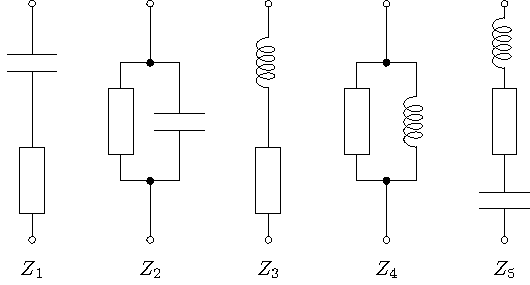
\includegraphics[scale=1.1]{elektroPhilip1.pdf}
    \caption{5 Exemplarische Zweipole mit den Impedanzen $Z_1$ bis $Z_5$}
\end{figure}
%
% Ne Figure mit 4 Subfigures, wenn du dass hinbekommst.
% Ne RC Reihe, Ne RC Parallel, Ne RL Reihe, Ne RL Parallel, ne RLC Reihe. (Z_1 - Z_5)
%
Für jede dieser Schaltungen lässt sich recht einfach die Gesamtimpedanz berechnen, aus der wir dann
die anderen Größen erhalten, welche wir schließlich Interpretieren wollen.
Es sei $R=\SI{1}{\kilo\ohm},\, C=\SI{1}{\nano\farad},\, L=\SI{1}{\henry}$ und $\omega = 1,10^3,10^{9} \si{Hz}$.
% normale werte, eisenkernspule
In dem selben Stil lassen sich auch die Impedanzen von komplexeren Kombinationen
von Reihen- und Parallelschaltungen berechnen. Auch die Lösung des linearen Gleichungssystems aus den Kirchhoffschen Gesetzen für noch kompliziertere Schaltungen geht analog zur Behandlung von Schaltungen aus Widerständen.
\begin{align*}
    && &\qquad \omega = \SI{1}{\Hz} &&\qquad \omega = \SI{1e3}{\Hz} &&\qquad \omega = \SI{1e9}{\Hz} \\
    Z_1 &= R + \ic 
    &&= (10^3 - 10^9 \imu)\,\si{\ohm} &&=(10^3 - 10^6 \imu)\,\si{\ohm} &&=(10^3 - \imu)\,\si{\ohm} \\
    Z_2 &= R \parallel \ic = \frac{1}{\frac{1}{R} + \imu \omega C}
    &&\approx (10^3 - 10^{-3} \imu)\,\si{\ohm} &&\approx(10^3 - \imu)\,\si{\ohm} &&\approx(10^{-3} - \imu)\,\si{\ohm} \\
    Z_3 &= R + \il 
    &&= (10^3 - \imu)\,\si{\ohm} &&=(10^3 - 10^3 \imu)\,\si{\ohm} &&=(10^3 - \imu)\,\si{\ohm} \\
    Z_4 &= R \parallel \il = \frac{1}{\frac{1}{R} + \frac{1}{\il}} 
    &&\approx (10^{-3} - \imu)\,\si{\ohm} &&\approx(500 - 500 \imu)\,\si{\ohm} &&\approx(10^3 - 10^{-3}\imu)\,\si{\ohm} \\
    Z_5 &= R + \il + \ic 
    &&= (10^3 - 10^9\imu)\,\si{\ohm} &&\approx(10^3 - 10^6 \imu)\,\si{\ohm} &&=(10^3 + 10^9\imu)\,\si{\ohm} 
\end{align*}
% wär irgendwie cool, wenn wir |Z_n| über w plotten könnten. Bock das zu machen?
Man sieht das typische Verhalten der passiven Bauteile. Der Scheinwiderstand einer Spule verringert 
sich für geringere Frequenzen, der eines Kondensators für hohe Frequenzen.
Für RC/RL Reihenschaltungen führt dies zu einer Frequenzabhängigen Phasendifferenz $\arctan(\tfrac{X_{C/L}}{R})$, der Scheinwiderstand fällt/wächst mit steigender Frequenz, bleibt aber strikt größer als $R$.
Für die RC/RL Parallelschaltungen verhält es sich entgegengesetzt analog.
Bemerkenswert ist dabei, dass dadurch der Wirkwiderstand reduziert werden kann.
$Z_5$ stellt die Gesamtreihenschaltung aus $R$, $C$ und $L$ dar, und besitzt einen minimalen Scheinwiderstand von $R$ und Blindwiderstand von $0$ bei einer Grenzfrequenz $f_g = 10^{4.5}\si{\hertz}$, bei der sich die beiden Blindwiderstandsanteile genau aufheben.
Legt man z.B. die Amplitude der Spannung über die beiden Pole fest, so kann man mit diesen Schaltungen Strom so steuern, dass er nur bei hohen Frequenzen, niedrigen Frequenzen, mittleren Frequenzen oder alles außer mittleren Frequenzen fließt. Betrachtet man den Spannungsanteil, der bei verschiedenen Frequenzen über ein Teilbauteil abfällt und nimmt diesen als Output, so kann man damit auch Spannungen über die Frequenz regeln. Man siehe Kapitel (?).
%%% ICH HAB VERGESSEN WIE LABELS WORKEN UND BIN FAUL

Überlegt man sich jedoch, wie sich die LC-Kreise wie $Z_5$ ohne Widerstand speziell bei $f_g$ verhalten, dann kommt man zu Schwingkreisen.

\begin{figure}[h!]
    \centering
    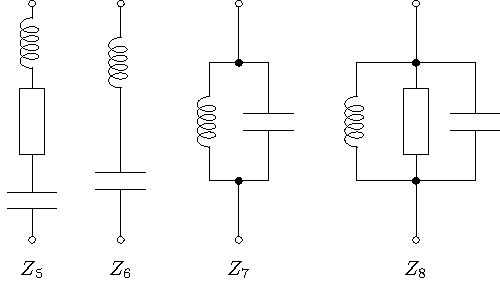
\includegraphics[scale=1.1]{elektroPhilip2.pdf}
    \caption{Zweipole mit Resonanzverhalten mit Impedanzen $Z_5$ bis $Z_8$}
\end{figure}
%
% Ne Figure mit 4 Subfigures, wenn du dass hinbekommst.
% die selbe RLC Reihe, Ne LC Reihe, Ne RLC Parallel, Ne RLC Parallel. (Z_5 - Z_8)
%
\begin{align*}
    \qquad&&Z_5 &= R + \il + \ic & \xrightarrow{R \,\rightarrow \,\SI{0}{\ohm}} && \il + \ic &= Z_6 
    &&\qquad\\
    \qquad&&Z_8 &= R \parallel \il \parallel \ic & \xrightarrow{R \,\rightarrow \,\SI{0}{\ohm}} && \il \parallel \ic &= Z_7 &&\qquad\\
\end{align*}
In Schaltung $Z_5$ und $Z_6$ verringert sich der Blindwiderstand nach der Wechselstromrechnung bei höheren Frequenzen auf 0 und steigt dann bei noch höheren Frequenzen wieder vom Betrag her an.
Warum? Weil sie bei dieser Frequenz einen (un)gedämpften Schwingkreis darstellt, welcher mit Resonanzfrequenz betrieben wird, weswegen die Schaltung keine Arbeit verrichtet, da Sie sich von selber in Schwingung befindet.
Schaltungen $Z_7$ und $Z_8$ beschreiben den selben Schwingkreis, an welchen nun allerdings von außen 
Spannung angelegt wird. diese Spannung erzeugt bei im Ungedämpften Kreis bei der Resonanzfrequenz jedoch nur einen Fluss innerhalb der Schaltung, da der Kondensator genau den Strom nimmt, den die Spule gibt.
% DIE DUDS KÖNNEN SCHWINGKREISE; DESWEGEN ERKLÄR ICH DAS HIER NICH LANG UND BREIT
Die Wechselstromrechenmethode ist hier also in der Lage, die Effekte solcher Schwingungen richtig vorherzusagen.
\begin{align*}
    Z_6 &\stackrel{!}{=} 0 &\implies&& \il &= -\ic &\implies&& \omega^2 &= \frac{1}{LC} \eqqcolon f_{g}^2\\
    Z_8 &\stackrel{!}{=} \infty &\implies&& \frac{1}{\imu \omega L} &= -\imu \omega C &\implies&& \omega^2 &= \frac{1}{LC} = f_{g}^2\\
\end{align*}

\subsection*{Vierpole}
\begin{figure}[h!]
    \centering
    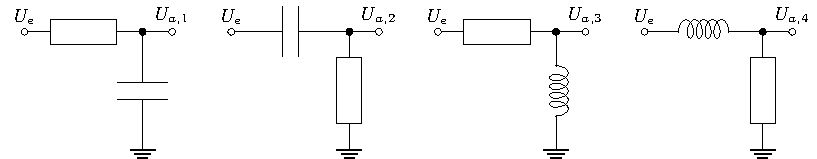
\includegraphics[scale=1.1]{elektroPhilip3.pdf}
    \caption{Die vier typischen $RC$- oder $RL$-Filtervierpole}
\end{figure}
%
% Ne Figure mit 4 Subfigures, wenn du dass hinbekommst.
% $RC$-Hochpass,$RC$-Tiefpass,$RL$-Tiefpass,$RL$-Hochpass.
% mit U_e als Eingangsspannung und U_a als Ausgangsspannung.
In der Abbildung sieht man (v.l.n.r.) einen $RC$-Hochpass, einen $RC$-Tiefpass, einen $RL$-Tiefpass
und einen $RL$-Hochpass.
Diese können wir schlicht als Spannungsteiler auffassen und deren Ausgangspannung in Abhängigkeit der Eingangsspannung und der Frequenz bestimmen\footnote{
Man siehe auch \url{https://physik.uni-greifswald.de/storages/uni-greifswald/fakultaet/mnf/physik/Studium/Elektronik/elektronik-vorlesung.pdf}, Kapitel 4 für eine umfassendere und tiefergehende Behandlung von Schaltungen mit passiven Bauelementen}.
Man definiert $\Omega_C = \omega RC, \, \Omega_L = \omega\frac{L}{R}$. Dies entspricht einer auf die Grenzfrequenz genormten Einheitslosen Kreisfrequenz.
\begin{align}
    \text{RC-Hochpass:} && 
    \frac{U_{a,1}}{U_e} = \frac{R}{X_C + R}   &=
        \frac{1}{1 - \imu \frac{1}{\omega RC}} =
        \frac{\imu \Omega_C}{1 + \imu \Omega_C} &\quad
        \abs{\frac{U_{a,1}}{U_e}} &= \frac{\Omega_C}{\sqrt{1+\Omega_C^2}}\\
    \text{RC-Tiefpass:} && 
    \frac{U_{a,2}}{U_e} = \frac{X_C}{X_C + R} &= 
        \frac{1}{1 + \imu \omega RC} =
        \frac{1}{1 + \imu \Omega_C} &\quad
        \abs{\frac{U_{a,2}}{U_e}} &= \frac{1}{\sqrt{1+\Omega_C^2}}\\
    \text{RL-Tiefpass:} && 
    \frac{U_{a,3}}{U_e} = \frac{R}{X_L + R} &= 
        \frac{1}{1 + \imu  \frac{\omega L}{R}} =
        \frac{1}{1 + \imu \Omega_L} &\quad
        \abs{\frac{U_{a,3}}{U_e}} &= \frac{1}{\sqrt{1+\Omega_L^2}}\\
    \text{RL-Hochpass:} && 
    \frac{U_{a,4}}{U_e} = \frac{X_L}{X_L + R} &= 
        \frac{1}{1 - \imu \frac{R}{\omega L}} =
        \frac{\imu \Omega_L}{1 + \imu \Omega_L} &\quad
        \abs{\frac{U_{a,4}}{U_e}} &= \frac{\Omega_L}{\sqrt{1+\Omega_L^2}} 
\end{align}
Der Betrag der Übertragsfunktion stellt hierbei das Verhältnis der Eingangsspannungsamplitude und der Ausgangsspannungsamplitude dar. Eine Phasenverschiebung existiert, ist aber hier nicht weiter wichtig.

Die Tiefpässe skalieren invers proportional zu $\sqrt{1 + \Omega^2}$. Da $\Omega \propto \omega$ steigt die Wurzel an, für große Frequenzen grob linear, für kleine Frequenzen weniger.
Die Übertragsfunktion ist also maximal und gleich 1 bei $\Omega = 1$ und fällt dann immer weiter, um sich bei großen Frequenzen wie $1/\Omega$ gegen 0 zu nähern.
Die Hochpässe besitzen die gleiche Übertragsfunktion, noch skaliert mit $\Omega$.
Für geringe $\Omega$ ist also auch die Übertragsfunktion klein, während sie sich bei großen Frequenzen an 1 annähert.
Zu beachten ist dabei das Verhalten der Pässe bei inverser normierter Kreisfrequenz.
\begin{align}
    \abs{\frac{U_{a,\text{Tief}}(U_e, \frac{1}{\Omega})}{U_e}} &= \frac{1}{\sqrt{1+\frac{1}{\Omega^2}}}
    = \frac{1}{\sqrt{\frac{1}{\Omega^2}}\sqrt{\Omega^2+1}} = \frac{\Omega}{\sqrt{\Omega^2+1}} 
    = \abs{\frac{U_{a,\text{Hoch}}(U_e, \Omega)}{U_e}}\\
    \abs{\frac{U_{a,\text{Hoch}}(U_e, \frac{1}{\Omega})}{U_e}} &
    = \frac{\frac{1}{\Omega^2}}{\sqrt{1+\frac{1}{\Omega^2}}}
    = \frac{1}{\sqrt{{\Omega^2}}\sqrt{1+\frac{1}{\Omega^2}}} = \frac{1}{\sqrt{\Omega^2+1}} 
    = \abs{\frac{U_{a,\text{Tief}}(U_e, \Omega)}{U_e}}
\end{align}
Ein solcher Hochpass verhält sich also bezüglich der Amplitudenskalierung bei einer Frequenz $1/\Omega$ genau so, wie der äquivalente Tiefpass bei $\Omega$.
Die Phasenverschiebung ist jedoch umgekehrt. Eine Phasenerhöhung $\Delta \phi$ beim Hochpass bei $1/\Omega$ entspricht einer genau entgegengesetzten Phasenverringerung um $-\Delta \phi$ beim Tiefpass bei $\Omega$.
%
% ggf. ÜA: Beweise das.
%
\end{document}
    